
%% \begin{figure*}
%%   \centering
%%   \subfloat[Optimizer Sensitivity]{
%%     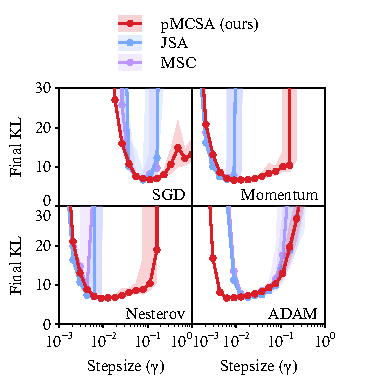
\includegraphics[scale=1.0]{figures/stepsize_01.pdf}
%%   } \\
%%   \subfloat[Gradient Variance]{
%%     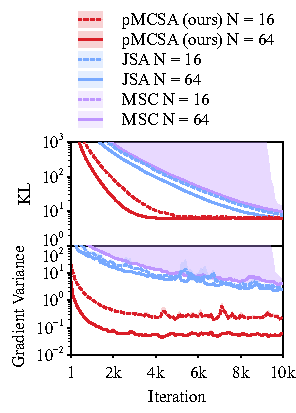
\includegraphics[scale=1.0]{figures/gaussian_01.pdf}
%%   }
%%   \caption{\textbf{Optimizer stepsize (\(\gamma\)) versus final KL. pMCSA is the least sensitive to optimizer hyperparameters and results in stable convergence.}
%%       The final KL is obtained at the \(10^4\)th iteration.
%%       The target distribution is a 100-D Gaussian with \(\nu = 500\).
%%       The error bands are the 80\% quantiles while the solid lines are the median of 20 replications.
%%   }
%% \end{figure*}

%\vspace{-0.1in}
\section{Evaluations}\label{section:eval}
\vspace{-0.1in}
\subsection{Experimental Setup}
%\vspace{-0.05in}
\paragraph{Implementation}
For the realistic experiments, we implemented MCSA methods on top of the Turing~\citep{ge2018t} probabilistic programming framework.%\footnote{Available at \url{https://github.com/Red-Portal/KLpqVI.jl}}.
For the variational family, we use diagonal multivariate Gaussians with the support transformation of~\citet{JMLR:v18:16-107}.
We use the ADAM optimizer by~\citet{kingma_adam_2015} with a stepsize of 0.01 in all experiments.
The budget is set to \(N=10\) for all experiments unless specified.

\begin{figure*}[t]
  \vspace{-2ex}
  \centering
%%   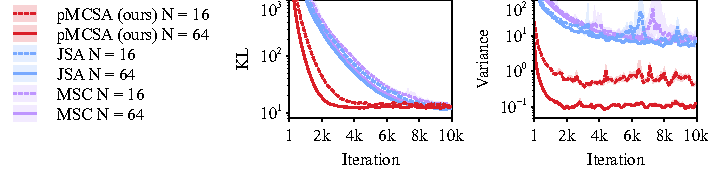
\includegraphics[scale=1.0]{figures/gaussian_02.pdf}
  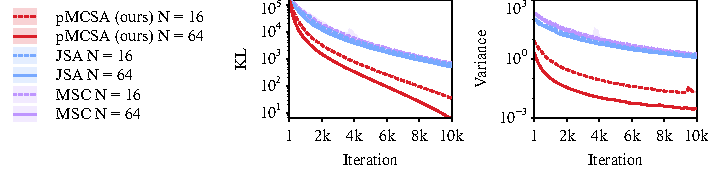
\includegraphics[scale=1.0]{figures/gaussian_03.pdf}
  %\vspace{-0.08in}
  \caption{\textbf{Gradient variance versus iteration and computational budget (\(N\)).
      pMCSA not only achieves the least gradient variance, but its variance also scales better with \(N\).
    }
    The colors range from light (\(N=2^3\)) to dark (\(N=2^7\)) representing the computational budgets \(N \in [2^3, 2^4, 2^5, 2^6, 2^7]\).
    The target distribution is a 50-D multivariate Gaussian with \(\nu = 500\).
    The error bands are the 80\% quantiles obtained from 8 replications.
  }\label{fig:gaussian}
\end{figure*}

\begin{figure*}[t]
  \vspace{-2ex}
  \centering
  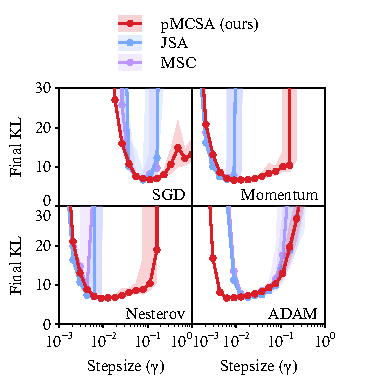
\includegraphics[scale=1.0]{figures/stepsize_01.pdf}
  %\vspace{-0.05in}
  \caption{\textbf{Optimizer stepsize (\(\gamma\)) versus final KL.
      pMCSA is the least sensitive to optimizer hyperparameters and results in stable convergence.}
      The final KL is obtained at the \(10^4\)th iteration.
      The target distribution is a 100-D Gaussian with \(\nu = 500\).
      The error bands are the 80\% quantiles, while the solid lines are the median of 20 replications.
  }\label{fig:stepsize}
  \vspace{-2ex}
\end{figure*}


\vspace{-0.1in}
\paragraph{Baselines}
We compare
\begin{enumerate*}[label=\textbf{(\roman*)}]
  \item \textbf{pMCSA} (ours,~\cref{section:pmcsa}),
  \item \textbf{JSA}~\citep{pmlr-v124-ou20a},
  \item \textbf{MSC}~\citep{NEURIPS2020_b2070693},
  \item MSC with with Rao-Blackwellization (\textbf{MSC-RB},~\citealt{NEURIPS2020_b2070693}), and
  %\item adaptive importance sampling (IS) with the self-normalized IS estimator (\textbf{SNIS},~\citealt{robert_monte_2004}), and
  \item evidence lower-bound maximization (\textbf{ELBO},~\citealt{pmlr-v33-ranganath14, JMLR:v18:16-107}) with the path derivative estimator~\citep{NIPS2017_e91068ff}.
\end{enumerate*}

\vspace{-0.1in}
\subsection{Simulations}\label{section:simulation}
%\vspace{-0.1in}
\paragraph{Setup}
First, we verify our theoretical analysis on multivariate Gaussians with full-rank covariances sampled from Wishart distribution with \(\nu\) degrees of freedom (values of \(\nu\) are in the figure captions).
This problem is challenging since an IMH (used by pMCSA, JSA) or CIS (used by MSC, MSC-RB) kernel with a diagonal Gaussian proposal will mix slowly due to a large \(w^*\).
% Since the exact KL divergence between the target and the varitional approximation is available, accurate evaluation is possible.

\vspace{-0.1in}
\paragraph{Gradient Variance}
We evaluate our theoretical analysis of the gradient variance.
The variance is estimated from \(512\) independent Markov chains using the parameters generated by the main MCSA procedure.
The estimated variances are shown in \cref{fig:gaussian}.
We make the following observations:
\begin{enumerate*}[label=\textbf{(\roman*)}]
  \item pMCSA has the lowest variance overall, and it consistently benefits from increasing \(N\).
  \item MSC does not benefit from increasing \(N\) whatsoever.
    
  \item \textcolor{blue}{
    MSC-RB does not benefit much from increasing \(N\) until the divergence of \(q\left(\cdot; \vlambda\right)\) has become small.
    }
  \item JSA does not benefit from increasing \(N\) until \(q\left(\cdot; \vlambda\right)\) has sufficiently converged (when \(w^*\) has become small).
\end{enumerate*}
These results confirm our theoretical results in~\cref{section:comparison,section:pmcsa}.


\begin{table*}
  \vspace{-0.1in}
  \centering
  \caption{Test Log Predictive Density on Bayesian Neural Network Regression}\label{table:bnn}
  \vspace{-0.05in}
  \setlength{\tabcolsep}{2pt}
  \begin{threeparttable}
  \begin{tabular}{lrrrcccccc}
    \toprule
    & \multicolumn{1}{c}{\multirow{2}{*}{\(D_{\mathcal{\vlambda}}\)}} & \multicolumn{1}{c}{\multirow{2}{*}{\(D_{\mathcal{\vx}}\)}} &  \multicolumn{1}{c}{\multirow{2}{*}{\(N_{\text{train}}\)}} & \multicolumn{2}{c}{\multirow{1}{*}{ELBO}} & \multicolumn{4}{c}{MCSA Variants} \\\cmidrule(lr){5-6}\cmidrule(lr){7-10}
  & & & & {\footnotesize\(N=1\)} & {\footnotesize\(N=10\)} & \multicolumn{1}{c}{\multirow{1}{*}{\footnotesize{\textbf{pMCSA{\scriptsize\,(ours)}}}}} & \multicolumn{1}{c}{\multirow{1}{*}{\footnotesize{JSA}}} & \multicolumn{1}{c}{\multirow{1}{*}{\footnotesize{CIS}}} & \multicolumn{1}{c}{\multirow{1}{*}{\footnotesize{CIS-RB}}}\\
    \midrule
    \textsf{yacht} & 403 & 6 & 277 & {\bf-2.45 {\scriptsize{\(\pm 0.01\)}}} & {\bf-2.44 {\scriptsize{\(\pm 0.01\)}}} & {\bf-2.49 {\scriptsize{\(\pm 0.01\)}}} & {-3.00 {\scriptsize{\(\pm 0.05\)}}} & {-2.98 {\scriptsize{\(\pm 0.04\)}}} & {-2.98 {\scriptsize{\(\pm 0.04\)}}}\\
    \textsf{concrete} & 503 & 8 & 927 & {-3.25 {\scriptsize{\(\pm 0.01\)}}} & {\bf-3.24 {\scriptsize{\(\pm 0.01\)}}} & {\bf-3.20 {\scriptsize{\(\pm 0.01\)}}} & {-3.33 {\scriptsize{\(\pm 0.02\)}}} & {-3.32 {\scriptsize{\(\pm 0.02\)}}} & {-3.33 {\scriptsize{\(\pm 0.02\)}}}\\
    \textsf{airfoil} & 353 & 6 & 1352 & {-2.53 {\scriptsize{\(\pm 0.02\)}}} & {-2.56 {\scriptsize{\(\pm 0.02\)}}} & {\bf-2.27 {\scriptsize{\(\pm 0.02\)}}} & {-2.51 {\scriptsize{\(\pm 0.02\)}}} & {-2.53 {\scriptsize{\(\pm 0.01\)}}} & {-2.51 {\scriptsize{\(\pm 0.01\)}}}\\
    \textsf{energy} & 503 & 9 & 691 & {-2.42 {\scriptsize{\(\pm 0.02\)}}} & {-2.40 {\scriptsize{\(\pm 0.02\)}}} & {\bf-1.92 {\scriptsize{\(\pm 0.03\)}}} & {-2.38 {\scriptsize{\(\pm 0.02\)}}} & {-2.37 {\scriptsize{\(\pm 0.02\)}}} & {-2.36 {\scriptsize{\(\pm 0.02\)}}}\\
    \textsf{boston} & 753 & 14 & 455 & {\bf-2.72 {\scriptsize{\(\pm 0.03\)}}} & {\bf-2.70 {\scriptsize{\(\pm 0.03\)}}} & {\bf-2.69 {\scriptsize{\(\pm 0.02\)}}} & {-2.82 {\scriptsize{\(\pm 0.02\)}}} & {-2.80 {\scriptsize{\(\pm 0.03\)}}} & {-2.78 {\scriptsize{\(\pm 0.02\)}}}\\
    \textsf{sml} & 1203 & 23 & 3723 & {-1.32 {\scriptsize{\(\pm 0.01\)}}} & {\bf-1.25 {\scriptsize{\(\pm 0.02\)}}} & {\bf-1.22 {\scriptsize{\(\pm 0.01\)}}} & {-1.72 {\scriptsize{\(\pm 0.01\)}}} & {-1.97 {\scriptsize{\(\pm 0.02\)}}} & {-1.95 {\scriptsize{\(\pm 0.02\)}}} \\
    \textsf{gas} & 6503 & 129 & 2308 & {\bf-0.06 {\scriptsize{\(\pm 0.01\)}}} & {\bf 0.13 {\scriptsize{\(\pm 0.03\)}}} & {-0.09 {\scriptsize{\(\pm 0.02\)}}} & {-0.47 {\scriptsize{\(\pm 0.03\)}}} & {-0.47 {\scriptsize{\(\pm 0.04\)}}} & {-0.50 {\scriptsize{\(\pm 0.03\)}}}\\
    \bottomrule
 \end{tabular}
  \begin{tablenotes}
    \item[1] {\footnotesize \(D_{\vlambda}\): Dimentionality of \(\vlambda\), \(D_{\vx}\): Number of features, \(N_{\text{train}}\): Number of training data points.}
    \item[2] {\footnotesize \(\pm\) denotes the 95\% bootstrap confidence intervals obtained from 80 repetitions.}
    \item[3] {\footnotesize Bolded numbers don't have enough evidence to be distinguished from the best performing method under a .05 significance threshold (Friedman test with Nemenyi post-hoc test,~\citealt{JMLR:v7:demsar06a})}.
  \end{tablenotes}
  \end{threeparttable}
  \vspace{-0.1in}
\end{table*}

%%% Local Variables:
%%% TeX-master: "master"
%%% End:


%\begin{wraptable}{r}{0.4\textwidth}
\begin{table*}[t]
  \centering
  \vspace{-2ex}
  \caption{Test Log Predictive Density on \textbf{Robust Gaussian Process Regression}}\label{table:gp}
  \vspace{-1ex}
  %\vspace{-0.05in}
  \setlength{\tabcolsep}{4pt}
  \begin{threeparttable}
  \begin{tabular}{lrrrccccc}
    \toprule
    & \multicolumn{1}{c}{\multirow{2}{*}{\footnotesize\(D_{\vlambda}\)}} & \multicolumn{1}{c}{\multirow{2}{*}{\(D_{\vx}\)}} &  \multicolumn{1}{c}{\multirow{2}{*}{\(N_{\text{train}}\)}} & \multicolumn{1}{c}{\multirow{1}{*}{ELBO}} & \multicolumn{4}{c}{MCSA Variants} \\\cmidrule(lr){5-5}\cmidrule(lr){6-9}
   & & & & \(N=1\) & \multicolumn{1}{c}{\multirow{1}{*}{\footnotesize\textbf{pMCSA{\scriptsize\,(ours)}}}} & \multicolumn{1}{c}{\multirow{1}{*}{\footnotesize{JSA}}} & \multicolumn{1}{c}{\multirow{1}{*}{\footnotesize{MSC}}} & \multicolumn{1}{c}{\multirow{1}{*}{\footnotesize{MSC-RB}}}\\
    \midrule
    \textsf{yacht} & 287 & 6 & 277 & {-3.63 {\scriptsize{\(\pm 0.02\)}}} & {\bf-3.31 {\scriptsize{\(\pm 0.04\)}}} & {\bf-3.29 {\scriptsize{\(\pm 0.05\)}}} & {\bf-3.25 {\scriptsize{\(\pm 0.04\)}}} & {\bf-3.27 {\scriptsize{\(\pm 0.05\)}}} \\
    \textsf{airfoil} & 353 & 6 & 1352 & {-3.14 {\scriptsize{\(\pm 0.01\)}}} & {\bf-2.63 {\scriptsize{\(\pm 0.01\)}}} & {-2.83 {\scriptsize{\(\pm 0.04\)}}} & {-2.77 {\scriptsize{\(\pm 0.02\)}}} & {\bf-2.73 {\scriptsize{\(\pm 0.02\)}}}\\
    \textsf{boston} & 472 & 13 & 455 & {\bf-2.98 {\scriptsize{\(\pm 0.01\)}}} & {\bf-2.96 {\scriptsize{\(\pm 0.02\)}}} & {\bf-3.00 {\scriptsize{\(\pm 0.03\)}}} & {\bf-3.00 {\scriptsize{\(\pm 0.03\)}}} & {\bf-2.96 {\scriptsize{\(\pm 0.03\)}}} \\
    \textsf{energy} & 703 & 8 & 691 & {-2.75 {\scriptsize{\(\pm 0.01\)}}} & {\bf-2.58 {\scriptsize{\(\pm 0.03\)}}} & {-2.78 {\scriptsize{\(\pm 0.04\)}}} & {-2.70 {\scriptsize{\(\pm 0.04\)}}} & {-2.72 {\scriptsize{\(\pm 0.05\)}}} \\
    \textsf{concrete} & 939 & 8 & 927 & {-3.68 {\scriptsize{\(\pm 0.01\)}}} & {\bf-3.49 {\scriptsize{\(\pm 0.01\)}}} & {-3.69 {\scriptsize{\(\pm 0.02\)}}} & {\bf-3.59 {\scriptsize{\(\pm 0.04\)}}} & {\bf-3.57 {\scriptsize{\(\pm 0.02\)}}} \\
    \textsf{wine} & 1454 & 11 & 1439 & {-1.02 {\scriptsize{\(\pm 0.01\)}}} & {\bf-0.94 {\scriptsize{\(\pm 0.02\)}}} & {-1.04 {\scriptsize{\(\pm 0.01\)}}} & {-1.00 {\scriptsize{\(\pm 0.02\)}}} & {-0.99 {\scriptsize{\(\pm 0.02\)}}} \\
    \textsf{gas} & 2440 & 128 & 2308 & {\bf{0.18} {\scriptsize{\(\pm 0.02\)}}} & {\bf-0.86 {\scriptsize{\(\pm 0.02\)}}} & {-1.10 {\scriptsize{\(\pm 0.03\)}}} & {-1.10 {\scriptsize{\(\pm 0.04\)}}} & {-1.06 {\scriptsize{\(\pm 0.02\)}}} 
    \\\bottomrule
  \end{tabular}
  \begin{tablenotes}
    \item[1] {\footnotesize \(D_{\vlambda}\): Dimentionality of \(\vlambda\), \(D_{\vx}\): Number of features, \(N_{\text{train}}\): Number of training data points.}
    \item[2] {\footnotesize \(\pm\) denotes the 95\% bootstrap confidence intervals obtained from 20 replications.}
    \item[3] {\footnotesize Bolded numbers don't have enough evidence to be distinguished from the best performing method under a .05 significance threshold (Friedman test with Nemenyi post-hoc test,~\citealt{JMLR:v7:demsar06a})}.
  \end{tablenotes}
  \end{threeparttable}
  \vspace{-2ex}
\end{table*}
%\end{wraptable}

%%% Local Variables:
%%% TeX-master: "master"
%%% End:


\vspace{-0.1in}
\paragraph{Robustness Against Optimizers}
Since the convergence of most sophisticated SGD optimizers has yet to be established for MCGD, we empirically investigate their effectiveness.
The results using SGD~\citep{robbins_stochastic_1951, bottou_optimization_2018a}, Momentum~\citep{polyak_methods_1964}, Nesterov~\citep{nesterov_method_1983}, ADAM~\citep{kingma_adam_2015}, and varying stepsizes are shown in~\cref{fig:stepsize}.
Clearly, pMCSA successfully converges for the broadest variety of optimizer settings.
Overall, most MCSA methods seem to be the most stable with ADAM, which points out that establishing the convergence of ADAM for MCGD will be a promising direction for future works.

%% \subsection{Hierarchical Logistic Regression}\label{section:logistic}
%% \vspace{-0.05in}
%% \paragraph{Experimental Setup}
%% We now perform logistic regression with the \texttt{Pima Indians} diabetes (\(\vz \in \mathbb{R}^{11}\),~\citealt{smith_using_1988}), \texttt{German credit} (\(\vz \in \mathbb{R}^{27}\)), and \texttt{heart disease} (\(\vz \in \mathbb{R}^{16}\),~\citealt{detrano_international_1989}) datasets obtained from the UCI repository~\citep{Dua:2019}.
%% 10\% of the data points were randomly selected in each of the 100 repetitions as test data.

% 
\begin{table*}
  \vspace{-0.2in}
  \centering
  \caption{Test Log Predictive Density on Gaussian Process Logistic Classification}\label{table:gp}
  \vspace{-0.05in}
  \setlength{\tabcolsep}{4pt}
  \begin{threeparttable}
  \begin{tabular}{lrrrrrr}
    \toprule
    & \multicolumn{1}{c}{\multirow{2}{*}{ELBO}} & \multicolumn{1}{c}{\multirow{1}{*}{\textbf{pMCSA}}} & \multicolumn{1}{c}{\multirow{2}{*}{JSA}} & \multicolumn{1}{c}{\multirow{2}{*}{CIS}} & \multicolumn{1}{c}{\multirow{2}{*}{CIS-RB}} & \multicolumn{1}{c}{\multirow{2}{*}{SNIS}} \\
    & & \multicolumn{1}{c}{\textbf{(ours)}} & & & & \\
    \midrule
    \textsf{sonar} & {-0.69 {\scriptsize{\(\pm 0.00\)}}} & {\bf-0.68 {\scriptsize{\(\pm 0.00\)}}} & {\bf-0.68 {\scriptsize{\(\pm 0.00\)}}} & {\bf-0.68 {\scriptsize{\(\pm 0.00\)}}} & {\bf-0.68 {\scriptsize{\(\pm 0.00\)}}} & {-0.69 {\scriptsize{\(\pm 0.00\)}}} \\
    \textsf{ionosphere} & {-0.36 {\scriptsize{\(\pm 0.01\)}}} & {\bf-0.35 {\scriptsize{\(\pm 0.01\)}}} & {\bf-0.35 {\scriptsize{\(\pm 0.01\)}}} & {\bf-0.35 {\scriptsize{\(\pm 0.01\)}}} & {\bf-0.35 {\scriptsize{\(\pm 0.01\)}}} & {\bf-0.35 {\scriptsize{\(\pm 0.01\)}}} \\
    \textsf{breast} & {\bf-0.10 {\scriptsize{\(\pm 0.00\)}}} & {-0.11 {\scriptsize{\(\pm 0.01\)}}} & {-0.14 {\scriptsize{\(\pm 0.01\)}}} & {-0.14 {\scriptsize{\(\pm 0.00\)}}} & {-0.14 {\scriptsize{\(\pm 0.01\)}}} & {-0.14 {\scriptsize{\(\pm 0.01\)}}} \\
    \textsf{heart} & {-0.44 {\scriptsize{\(\pm 0.01\)}}} & {\bf-0.43 {\scriptsize{\(\pm 0.01\)}}} & {\bf-0.43 {\scriptsize{\(\pm 0.01\)}}} & {\bf-0.43 {\scriptsize{\(\pm 0.01\)}}} & {\bf-0.43 {\scriptsize{\(\pm 0.01\)}}} & {-0.44 {\scriptsize{\(\pm 0.01\)}}} \\
    \textsf{german} & {\bf-0.48 {\scriptsize{\(\pm 0.01\)}}} & {-0.49 {\scriptsize{\(\pm 0.01\)}}} & {-0.50 {\scriptsize{\(\pm 0.01\)}}} & {-0.50 {\scriptsize{\(\pm 0.01\)}}} & {-0.51 {\scriptsize{\(\pm 0.02\)}}} & {-0.49 {\scriptsize{\(\pm 0.01\)}}} \\
    \textsf{australian} & {\bf-0.21 {\scriptsize{\(\pm 0.01\)}}} & {\bf-0.21 {\scriptsize{\(\pm 0.01\)}}} & {\bf-0.21 {\scriptsize{\(\pm 0.01\)}}} & {\bf-0.21 {\scriptsize{\(\pm 0.01\)}}} & {-0.22 {\scriptsize{\(\pm 0.01\)}}} & {\bf-0.21 {\scriptsize{\(\pm 0.01\)}}} \\\bottomrule
  \end{tabular}
  \begin{tablenotes}
    \item[]{\footnotesize \(\pm\) denotes the 95\% bootstrap confidence intervals obtained from 20 repetitions.}
  \end{tablenotes}
  \end{threeparttable}
  \vspace{-0.15in}
\end{table*}

%%% Local Variables:
%%% TeX-master: "master"
%%% End:


%% %

%%   \vspace{-0.1in}
%% \paragraph{Inclusive KL v.s. Exclusive KL}
%% While both ELBO and par.-IMH showed similar numerical performance, they chose different optimization paths in the parameter space.
%% This is shown in~\cref{fig:logistic}.
%% While the test accuracy suggests that ELBO converges quickly around \(t=2000\) (\cref{fig:german_acc}), in terms of uncertainty estimate, it takes much longer to converge (\cref{fig:german_lpd}).
%% This shows that inclusive KL minimization chooses a path that has better density coverage as expected.

  \vspace{-0.1in}
\subsection{Bayesian Neural Network Regression}\label{section:bnn}
  \vspace{-0.07in}
\looseness=-1
\paragraph{Setup}
For realistic experiments, we train Bayesian neural networks (BNN, \citealt{neal_bayesian_1996}) for regression.
We use datasets from the UCI repository~\citep{Dua:2019} with 90\% random train-test splits.
We run all methods with \(T=5\cdot10^4\) iterations.
For the model, we use the priors and forward propagation method of~\citet{pmlr-v37-hernandez-lobatoc15} with a \(50\)-unit hidden layer (see \cref{section:model_bnn}).
% \looseness=-1

\vspace{-0.1in}
\paragraph{Results}
The results are shown in~\cref{table:bnn}.
pMCSA achieves the best performance compared to all other MCSA methods.
Also, its overall performance is comparable to exclusive KL minimization methods (ELBO) unlike other MCSA methods.
Furthermore, on \textsf{airfoil} and \textsf{energy}, pMCSA improves over ELBO by 0.29 \texttt{nat} and 0.48 \texttt{nat}.
%
\begin{wrapfigure}[12]{r}{0.5\textwidth}
  \vspace{-4ex}
  \centering
  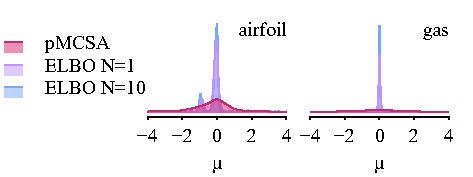
\includegraphics[scale=0.9]{figures/pruning_01.pdf}
  \vspace{-2ex}
  \caption{\textbf{
      Distribution of the variational posterior mean of the BNN weights.
      pMCSA restuls in significantly less pruning.
    }
    The density was estimated with a Gaussian kernel and the bandwidth was selected with Silverman's rule.
  }\label{fig:gaussian}
\end{wrapfigure}
%
Even on \textsf{gas} where pMCSA did not beat ELBO, its performance is comparable, and it dominates all other MCSA methods by roughly 0.4 \texttt{nat}.
Additional experimental results can be found in~\cref{section:bnn_additional}

\vspace{-6ex}
\textcolor{blue}{
\paragraph{Weight Pruning}
For BNNs, ELBO maximization has recently been dis to result in many of the weights being concentrated around zero.
For MCSA, 
This suggests that weight pruning is an artifact of using exclusive KL minimization rather
For BNNs, ELBO maximization has recently been dis to result in many of the weights being concentrated around zero.
}

\vspace{-0.1in}
\subsection{Robust Gaussian Process Regression}\label{section:bgp}
\vspace{-0.07in}
\paragraph{Setup}
We train Gaussian processes (GP) with a Student-T likelihood for robust regression.
We use datasets from the UCI repository~\citep{Dua:2019} with 90\% random train-test splits.
We use the Mat\'ern 5/2 covariance kernel with automatic relevance determination~\citep{neal_bayesian_1996} (see \cref{section:model_rgp}).
We run all methods with \(T=2\cdot10^4\) iterations.
For prediction, we use the mode of \(q\left(\cdot; \vlambda\right)\) for the hyperparameters and marginalize the latent function over \(q\left(\cdot; \vlambda\right)\)~\citep{rasmussen_gaussian_2006}.
We consider ELBO with only \(N=1\) since differentiating through the likelihood makes its per-iteration cost comparable to MCSA methods with \(N=10\).

\vspace{-0.1in}
\paragraph{Results}
The results are shown in~\cref{table:gp}.
Except for \textsf{gas}, pMCSA achieves better performance than all other methods.
This suggests that, overall, the exclusive KL may be less effective for GP posteriors.
Although ELBO achieves the best performance on \textsf{gas}, pMCSA dominates other MCSA methods.
Our encouraging regression results suggest that incorporating methods such as inducing points~\citep{NIPS2005_4491777b} into MCSA may lead to an important new class of GP models.
Additional experimental results can be found in~\cref{section:gp_additional}.

%%% Local Variables:
%%% TeX-master: "master"
%%% End:
